% Format teze zasnovan je na paketu memoir. Prilikom
% zadavanja klase memoir, navedenim opcijama se podešava
% veličina slova (12pt) i jednostrano štampanje (oneside).
\documentclass[12pt,oneside]{memoir}

% Paket koji definiše sve specifičnosti mastera Matematičkog fakulteta
\usepackage{matfmaster}

% Paket koji obezbeđuje ispravni prikaz ćiriličkih italik slova
\usepackage{cmsrb}

% Ostali paketi koji se koriste u dokumentu
\usepackage{listings} % listing programskog koda

\usepackage{CJKutf8}

% Komanda za ispis (npr. caption) u dva reda
\newcommand{\dvareda}[2][c]{\begin{tabular}[#1]{@{}c@{}}#2\end{tabular}}

% Datoteka sa literaturom u BibTex tj. BibLaTeX/Biber formatu
\bib{hmm_vasovic}

% Ime kandidata na srpskom jeziku (u odabranom pismu)
\autor{Лазар М. Васовић}
% Naslov teze na srpskom jeziku (u odabranom pismu)
\naslov{Скривени Марковљеви модели (\textit{HMM}) у биоинформатици}
% Godina u kojoj je teza predana komisiji
\godina{2021}
% Ime i afilijacija mentora (u odabranom pismu)
\mentor{др Јована \textsc{Ковачевић}, доцент\\ Универзитет у Београду, Математички факултет}
% Ime i afilijacija prvog člana komisije (u odabranom pismu)
\komisijaA{... ... \textsc{...}, ...\\ ..., ...}
% Ime i afilijacija drugog člana komisije (u odabranom pismu)
\komisijaB{... ... \textsc{...}, ...\\ ..., ...}
% Datum odbrane (obrisati ili iskomentarisati ako nije poznat)
\datumodbrane{септембар 2021.}

% Apstrakt na srpskom jeziku (u odabranom pismu)
\apstr{%
...
}

% Ključne reči na srpskom jeziku (u odabranom pismu)
\kljucnereci{биоинформатика, скривени Марковљеви модели (\textit{HMM})}

\begin{document}
\begin{CJK}{UTF8}{ipxm}
% ====================================================================
% Uvodni deo teze
\frontmatter
% ====================================================================
% Naslovna strana
\naslovna
% Strana sa podacima o mentoru i članovima komisije
\komisija
% Strana sa podacima o disertaciji na srpskom jeziku
\apstrakt
% Sadržaj teze
\tableofcontents*

% ====================================================================
% Glavni deo teze
\mainmatter
% ====================================================================

% ------------------------------------------------------------------------------
\chapter{Увод}
% ------------------------------------------------------------------------------
Биоинформатика је интердисциплинарна област која се бави применом рачунарских технологија у области биологије и сродних наука, са нагласком на разумевању биолошких података. Кључна особина јој је управо поменута мултидисциплинарност, која се може представити дијаграмом са слике \ref{fig:venn}.

\begin{figure}[!ht]
  \centering
  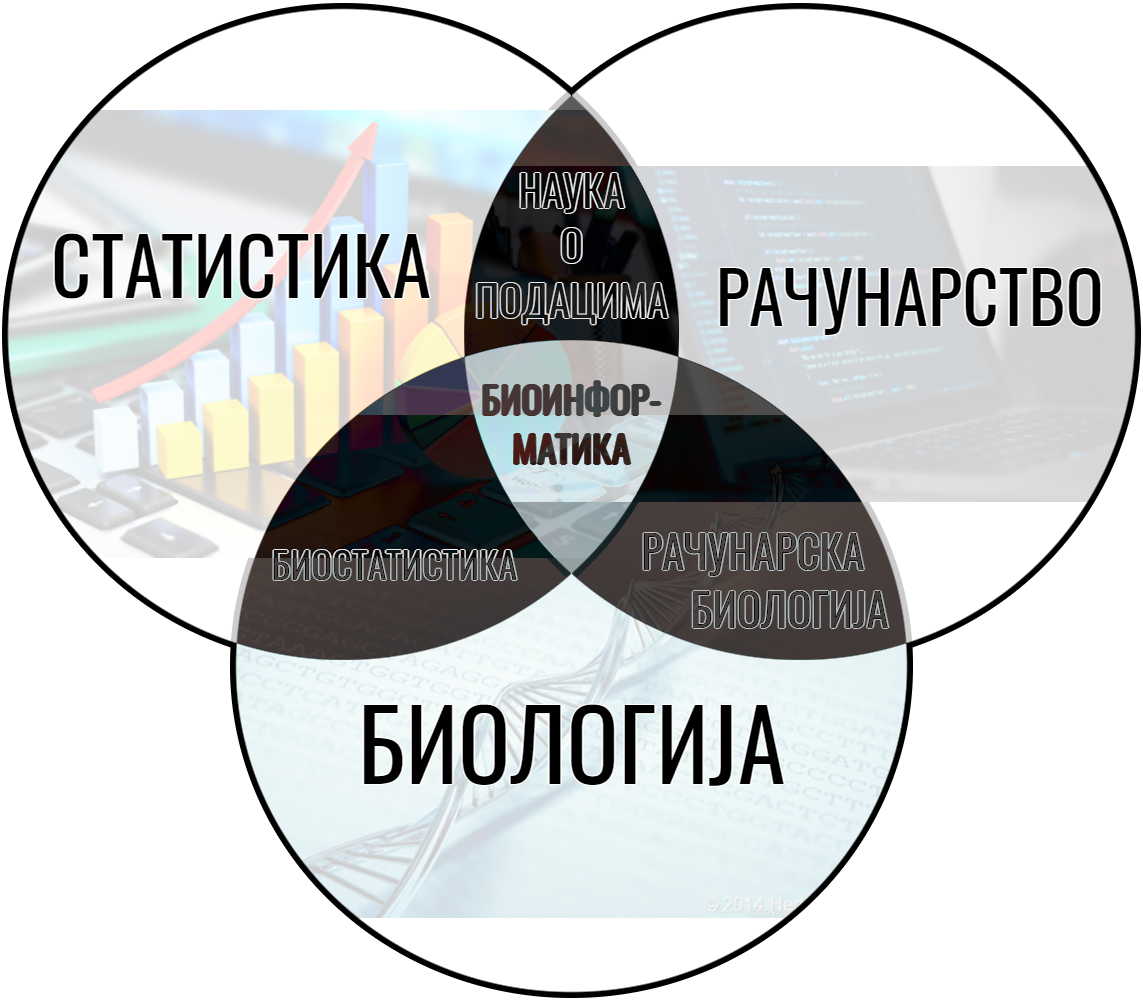
\includegraphics[width=0.75\textwidth]{bioinformatika.png}
  \caption{Венов дијаграм интердисциплинарности\cite{venn}}
  \label{fig:venn}
\end{figure}

Овако представљена, биоинформатика је заправо спој статистике, рачунарства и биологије -- сва три истовремено -- по чему надилази појединачне спојеве: биостатистику, науку о подацима и рачунарску биологију. Конкретно, статистички (математички) апаратат служи за рад са подацима, рачунарске технологије тај апарат чине употребљивијим, док биологија даје потребно доменско знање (разумевање) за рад са биолошким и сродним подацима. Иако се може рећи да је биоинформатика, у савременом смислу представљеном приказаним дијаграмом, релативно млада наука, брзо је постала популарна и многи су јој посветили пажњу или се њоме баве\cite{fauziyyah2019, cmero2015, ufpr}.

Међу познатим личностима из овога домена издвајају се научници Филип Компо (\textit{Phillip Compeau}) и Павел Певзнер (\textit{Pavel Pevzner}), аутори књиге \textit{Bioinformatics Algorithms: An Active Learning Approach}. Прво издање књиге изашло је 2014. године, а друго већ наредне, у два тома. Актуелно, треће издање, издато је 2018. године, у једном тому. Захваљујући динамичном и активном приступу биолошким проблемима и њиховим информатичким решењима, као и многим додатним материјалима за учење, књига се користи као уџбеник на више од сто светских факултета\cite{ba}. Међу њима је и Математички факултет Универзитета у Београду, односно на њему доступни мастер курс Увод у биоинформатику, а делови књиге користе се и у настави повезаног мастер и докторског курса Истраживање података у биоинформатици\cite{matf}.

Актуелна иницијатива на нивоу курса Увод у биоинформатику јесте израда електронског уџбеника, заснованог на поменутој књизи. Идеја је да заинтересовани студенти као мастер рад обраде по једно поглавље књиге, при чему обрада укључује писање текста на српском језику, али и имплементацију и евентуалну визуелизацију свих или макар већине пратећих алгоритама. Овај рад настао је управо у склопу представљене иницијативе, међу првима.

Уџбеник кроз једанаест глава обрађује разне теме које су занимљиве у оквиру биоинформатике: почетак репликације (алгоритамско загревање), генске мотиве (рандомизовани алгоритми), асемблирање генома (графовски алгоритми), секвенцирање антибиотика/пептида (алгоритми грубе силе), поређење и поравнање геномских секвенци (динамичко програмирање), блокове синтеније (комбинаторни алгоритми), филогенију (еволутивна стабла), груписање гена (кластеровање), проналажење шаблона (префиксна и суфиксна стабла), откривање гена и мутација секвенце (скривени Марковљеви модели), напредно секвенцирање пептида (рачунарска протеомика). Циљ овог рада је обрада десетог поглавља, заснованог на скривеним Марковљевим моделима\cite{compeau2015}.

Скривени Марковљев модел (у наставку углавном скраћено \textit{HMM}, према енгл. \textit{Hidden Markov Model}), укратко, представља статистички модел који се састоји из следећих елемената: скривених стања ($x_i$), опсервација ($y_i$), вероватноћа прелаза ($a_{ij}$), полазних ($\pi_i$) и излазних вероватноћа ($b_{ij}$), по примеру са слике \ref{fig:hmm}. \textit{HMM} се тако може схватити као коначни аутомат, при чему стања задржавају уобичајено значење, док вероватноће прелаза описују колико се често неки прелаз реализује. Полазне вероватноће одређују почетно стање. Овакав аутомат допуњује се идејом да свако стање са одређеном излазном вероватноћом емитује (приказује) неку опсервацију. Штавише, најчешће су само опсервације и познате у раду са \textit{HMM}, док се позадински низ стања погађа ("предвиђа"), па се управо зато стања и модели називају скривеним\cite{stamp2021}.

\begin{figure}[!ht]
  \centering
  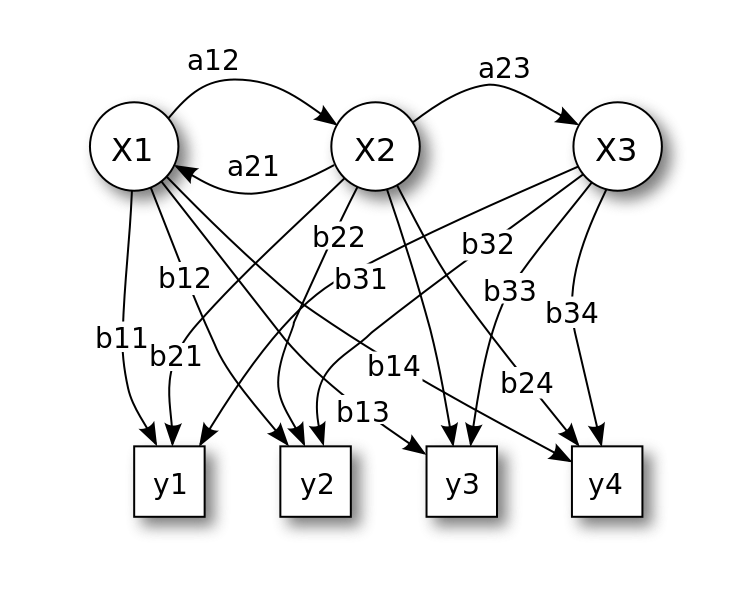
\includegraphics[width=0.75\textwidth]{hmm.png}
  \caption{Једноставан пример скривеног Марковљевог модела\cite{hmm}}
  \label{fig:hmm}
\end{figure}

У претходном пасусу су, наравно, скривени Марковљеви модели представљени малтене само концептуално, на високом нивоу. У наставку ће, међутим, они бити постепено уведени, заједно са мотивацијом за њихову употребу у виду биолошких проблема који се њима решавају. Према идеји електронског уџбеника, излагање ће пратити књигу \textit{Bioinformatics Algorithms: An Active Learning Approach}, а биће имплементирани и сви пратећи алгоритми. Сви кодови доступни су на \textit{GitHub} репозиторијуму у власништву аутора\cite{vasovich2021}.

% ------------------------------------------------------------------------------
\chapter{Мотивација}
% ------------------------------------------------------------------------------
За почетак, изложена је мотивација за употребу скривених Марковљевих модела у биоинформатици. Конкретно, представљена су два важна биолошка проблема која се њима могу решити и пратећи појмови из домена, као и једна историјски мотивисана вероватносна мозгалица. Ова глава, дакле, покрива прву петину обрађеног поглавља \textit{Chapter 10: Why Have Biologists Still Not Developed an HIV Vaccine? -- Hidden Markov Models}, и то тачно следеће поднаслове: \textit{Classifying the HIV Phenotype}, \textit{Gambling with Yakuza}, \textit{Two Coins up the Dealer’s Sleeve}, \textit{Finding CG-Islands}, и највећи део додатка из \textit{Detours}.

% Classifying the HIV Phenotype
\section{Погађање фенотипа}
\textit{HIV} је вирус хумане имунодефицијенције, један од најпознатијих вируса, који заражава људе широм света. Својим дугорочним деловањем доводи до смртоносног синдрома стечене имунодефицијенције, познатијег као сида или ејдс. Мада поједини аутори распрострањеност \textit{HIV}-а називају пандемијом, Светска здравствена организација означава је као "глобалну епидемију"\cite{who}.

Постојање \textit{HIV}-а званично је потврђено почетком осамдесетих година двадесетог века, мада се претпоставља да је са примата на људе прешао знатно раније. Недуго по овом открићу, тачније 1984, из америчког Министарства здравља и услуга становништву најављено је да ће вакцина бити доступна кроз наредне две године. Иако до тога није дошло, председник Бил Клинтон је 1997. потврдио да "није питање \textit{да ли} можемо да произведемо вакцину против сиде, већ је просто питање \textit{када} ће до тога доћи". Вакцина, међутим, ни данас није доступна, а многи покушаји су отказани након што се испоставило да кандидати чак повећавају ризик од инфекције код појединих испитаника.

Антивирусне вакцине најчешће се праве од површинских протеина вируса на који се циља, у нади да ће имунски систем, након вакцине, у контакту са живим вирусом знатно брже препознати протеине омотача вируса као стране и уништити их пре него што се вирус намножи у телу. \textit{HIV} је, међутим, карактеристичан по томе што врло брзо мутира, па су његови протеини изузетно варијабилни и није могуће научити имунски систем да исправно одреагује на све мутације. Штавише, може се десити да имунитет научи да исправно реагује само на једну варијанту вируса, а да реакција нема никаквог ефекта на остале варијанте. Овакав имунитет је лошији од имунитета који ништа не зна о вирусу, пошто не покушава да научи ништа ново, што је разлог већ поменуте ситуације да су код неких испитаника вакцине кандитати повећали ризик од заразе. Да ствар буде гора, \textit{HIV} брзо мутира и унутар једне особе, тако да је разлика у узорцима узетих од различитих пацијената увек значајна.

Када се све узме у обзир, као обећавајућа замисао за дизајн свеобухватне вакцине намеће се следећа идеја: идентификовати неки пептид који садржи најмање варијабилне делове површинских протеина свих познатих сојева \textit{HIV}-а и искористити га као основу вакцине. Ни то, међутим, није решење, пошто \textit{HIV} има још једну згодну способност: уме да се сакрије процесом гликолизације. Наиме, протеини омотача су махон гликопротеини, што значи да се након превођења за њих могу закачити многобројни гликански (шећерни) ланци. Овим процесом долази до стварања густог гликанског штита, који омета имунски систем у препознавању вируса. Све досад изнето утиче на немогућност прављења прикладне вакцине у скоријем времену.

Чак и ван контекста вакцине, мутације \textit{HIV}-а прилично су занимљиве за разматрање. Конкретно, илустративно је бавити се \textit{env} геном, чија је стопа мутације 1--2 \% по нуклеотиду годишње. Овај ген кодира два релативно кратка гликопротеина који заједно граде шиљак (спајк) омотача, део вируса задужен за улазак у људске ћелије. Мање важан део шиљка је гликопротеин \textit{gp41} ($\sim$ 345 аминокиселина), док је важнији гликопротеин \textit{gp120} ($\sim$ 480 аминокиселина). О варијабилности другог говори чињеница да на нивоу једног пацијента, у кратком року, скоро половина аминокиселина буде измењено позадинским мутацијама одговарајућег гена, као да је сасвим други протеин.

Ствари постају још занимљивије када се, поред генотипа вируса, разматра и његов фенотип. Примера ради, сваки вирус \textit{HIV}-а може се означити као изолат који ствара синцицијум или као изолат који га не ствара. Након уласка у људску ћелију, гликопротеини омотача могу да изазову спајање заражене ћелије са суседним ћелијама. Резултат тога је синцицијум -- нефункционална вишеједарна ћелијска (цитоплазматична) маса са заједничком ћелијском мембраном. Овакав изолат \textit{HIV}-а означава се као онај који ствара синцицијум и он се тим процесом знатно брже умножава, што даље значи да је опаснији и агресивнији, јер уласком у само једну ћелију убија многе друге у суседству. Одређивање тачног генотипа и погађање фенотипа важно је како би се пацијенту преписао најприкладнији коктел антивирусних лекова.

Испоставља се да је примарна структура гликопротеина \textit{gp120} важан суштински генотипски предиктор фенотипа \textit{HIV}-а. Наиме, узимајући у обзир само низ аминокиселина које чине \textit{gp120}, може се направити једноставан класификатор који погађа да ли проучавани изолат ствара синцицијум или не. Конкретно, научник Жан Жак де Јонг је 1992. анализирао вишеструко поравнање такозване \textit{V3} петље, издвојеног региона у оквиру \textit{gp120}, и формулисао правило 11/25. Према том правилу, сој \textit{HIV}-а највероватније ствара синцицијум уколико му се на 11. или 25. позицији у \textit{V3} петљи налазе аминокиселине аргинин (\textit{R}) или лизин (\textit{K}). Пример мотива \textit{V3} петље дат је на слици \ref{fig:motif}. Приметно је да су управо 11. и 25. позиција међу најваријабилнијим, те да удео критичних \textit{R} и \textit{K} на њима није претерано велик. Наравно, на фенотип утичу и многе друге позиције унутар \textit{gp120} и других протеина.

\begin{figure}[!ht]
  \centering
  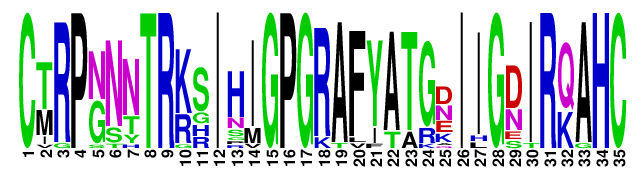
\includegraphics[width=0.75\textwidth]{motif.png}
  \caption{Мотив \textit{V3} петље из \cite{compeau2015} генерисан помоћу \cite{weblogo}}
  \label{fig:motif}
\end{figure}

За крај и поенту уводне приче о \textit{HIV}-у, остаје неразрешен још један веома значајан проблем. Како би се уопште разматрало предвиђање фенотипа на основу примарне структуре \textit{gp120}, неопходно је прво доћи до прецизног вишеструког поравнања различитих секвенци аминокиселина. Прво, поравнање мора бити хируршки прецизно, јер нпр. само једна грешка доводи до погрешног податка која вредност је на 11. и 25. позицији \textit{V3} петље. Следеће, неопходно је адекватно обрадити инсерције и делеције, што су врло честе мутације \textit{HIV}-а у многим регионима генома. На крају, потребно је на прави начин оценити квалитет поравнања, нпр. коришћењем различитих матрица скора за сваку појединачну позицију. Ово је донекле могуће урадити коришћењем техника представљених у петом поглављу (\textit{Chapter 5: How Do We Compare DNA Sequences? -- Dynamic Programming}), али уз два главна проблема: алгортми динамичког програмирања су високе сложености и са мање слободе код скорова, а притом не пресликавају најбоље суштину биолошког проблема класификације фенотипа у алгоритамски проблем (фале кораци након поравнања). Постоји, дакле, потреба за новом формулацијом која обухвата све што је потребно за статистички потковано поравнање секвенци.

% Finding CG-Islands
\section{Потрага за генима}
Познато је да геном чини тек мали део \textit{DNA} секвенце. Другим речима, \textit{DNA} добрим делом не кодира протеине. Стога је један од важних биолошких проблема управо проналажење места на којима се гени налазе. Прецизније, тражи се место где њихово преписивање (транскрипција) започиње.

Почетком двадесетог века, Фибус Левин открио је да \textit{DNA} чине четири нуклеотида, чији су главни део азотне базе: аденин (\textit{A}), цитозин (\textit{C}), гуанин (\textit{G}) и тимин (\textit{T}). У то време, међутим, није била позната тачна структура наследног материјала, штo је двострука завојница, коју су пола века касније открили Вотсон и Крик. Левин је, стога, сматрао да \textit{DNA} носи информације које су једнаке било којој четворословној азбуци, а додатно је сматрао и да је удео сваког од четири нуклеотида једнак. Занимљивост је да овај упрошћени модел одговара стању у савременој биоинформатици -- \textit{DNA} се углавном и посматра као секвенца нуклеотида, односно ниска над азбуком \{\textit{A}, \textit{C}, \textit{G}, \textit{T}\}.

Открићем тачке структуре допуњена је теза о једнаком уделу нуклеотида. Како су нуклеотиди на супротним ланцима упарени, њихов удео јесте врло сличан када се посматра целокупна \textit{DNA}. То, међутим, није случај када се посматра само један ланац, што је уобичајено у генетици и биоинформатици. Примера ради, удео гуанина и цитозина, који чине један базни пар, код људи је 42 \%, што је ипак статистички значајно мање од пола. На вишем нивоу гранулације, у случају да се посматрају само по две суседне базе, испоставља се да динуклеотиди \textit{CC}, \textit{CG}, \textit{GC}, \textit{GG} узимају сасвим различите уделе. Конкретно, иако би се очекивало да, под претпоставком равномерне расподеле, сваки од њих узима удео 4--5 \%, динуклетид \textit{CG} чини само 1 \% људског генома. Све ово значи да је \textit{DNA} секвенца ипак нешто даље од случајне.

Поставља се питање зашто је удео \textit{CG} тако мали. Одговор, међутим, није комплексан, поготову ако се додатно примети да је удео \textit{TG} нешто виши од очекиваног, а посебно у регионима у којима је удео \textit{CG} изразито мали. Разлог томе лежи у метилацији, најчешћој измени која природно настаје унутар \textit{DNA}. Поједини нуклеотиди, наиме, могу бити нестабилни, па се на њих лако накачи метил група ($CH_3$). Међу најнестабилнијим управо је цитозин иза ког следи гуанин, дакле \textit{C} из \textit{CG}. Метиловани цитозин даље се често спонтано деаминује у тимин, чиме динуклеотид \textit{CG} лако постаје \textit{TG}. Свеукупни резултат је да се \textit{CG} глобално појављује веома ретко, а \textit{TG} нешто чешће.

Метилација мења експресију суседних гена. Експресија оних гена чији су нуклеотиди у великој мери метиловани често је потиснута. Иако је сам процес метилације важан у току ћелијске диференцијације -- доприноси неповратној специјализацији матичних ћелија -- она углавном није пожељна у каснијем добу. Хиперметилација гена повезана је са различитим врстама рака. Стога је метилација врло ретка око гена, што значи да је на тим местима \textit{CG} знатно чешће. Овакви делови \textit{DNA} називају се \textit{CG} острвима или \textit{CpG} местима. Разлика у уделу динуклеотида у некодирајућим и регионима богатим генима дата је кроз табелу \ref{tab:cg}. Разлика у уделу \textit{CG} наглашена је црвеном бојом.

\begin{table}[h!]
  \centering
  \caption{\dvareda{Удео динуклеотида у једном ланцу људског \textit{X} хромозома\\-- лево у регионима \textit{CG} острва, а десно ван њих\cite{compeau2015}}}
  \begin{tabular}{c | c c c c | c c c c}
   & A & C & G & T & A & C & G & T\\ \hline
  A & 0,053 & 0,079 & 0,127 & 0,036 & 0,087 & 0,058 & 0,084 & 0,061\\
  C & 0,037 & 0,058 & \textcolor{red}{0,058} & 0,041 & 0,067 & 0,063 & \textcolor{red}{0,017} & 0,063\\
  G & 0,035 & 0,075 & 0,081 & 0,026 & 0,053 & 0,053 & 0,063 & 0,042\\
  T & 0,024 & 0,105 & 0,115 & 0,050 & 0,051 & 0,070 & 0,084 & 0,084\\
  \end{tabular}
  \label{tab:cg}
\end{table}

Закључак је, дакле, да се проблем потраге за генима може свести на проналажење \textit{CG} острва. Наиван приступ решавању овог проблема јесте употреба клизајућег прозора. Могао би се узети прозор фиксне величине и померати кроз \textit{DNA} секвенцу. Они прозори са натпросечним уделом \textit{CG} били би кандидати за \textit{CG} острва. Остаје, међутим, питање како одредити добру величину прозора, али и шта радити када преклапајући прозори нуде различиту класификацију подниза. И овде би боље било статистички потковано решење.

% Gambling with Yakuza
% Two Coins up the Dealer’s Sleeve
\section{Коцкање са јакузама}
Јакузе су припадници истоимене криминалне организације, традиционалног синдиката организованог криминала. Савремене јакузе потичу од јапанских путујућих коцкара, који су били распрострањени у осамнаестом веку. Једна од најпознатијих игара које су путујући коцкари организовали у својим импровизованим коцкарницама био је чо-хан (јап. 丁半, \textit{chō-han}), у буквалном преводу "пар-непар". Игра је сасвим једноставна -- претеча јакуза (крупије) баца две коцкице, док се играчи кладе да ли ће збир бити паран или непаран. Игра је такође праведна -- једнака је вероватноћа оба исхода парности.

До занимљивог тренутка долази када се из било ког разлога осетно више играча опклади на један од два могућа резултата. Тада би имало смисла да похлепни крупије, у жељи да заради (он узима проценат зараде победника), баца отежане коцкице, које ће са већом вероватноћом дати резултат који је добио мање опклада. Једноставности ради, уместо чо-хана ће у наставку бити разматрана једноставнија игра бацања новчића. У њој крупије баца новчић, а играчи се кладе да ли ће пасти писмо или глава. Она је знатно лакша за анализу, а суштина је иста и доводи до статистички поткованог решења у претходним поднасловима изложених биолошких и сродних проблема.

Крупијева превара у овом случају могла би бити употреба отежаног новчића, код кога исходи нису равномерно расподељени. Нека је познато да крупије има два новчића: један праведан и један отежан тако да на главу пада трипут чешће него на писмо. Циљ је за одређени низ исхода одредити да ли је настао бацањем праведног или отежаног новчића. Пажљивијом анализом проблема, испоставља се да је питање вара ли крупије лоше формулисано. Наиме, оба новчића могу да произведу било који низ исхода, па тако нпр. и отежани новчић може константно да пада на писмо. Иако дефинитивно није могуће са сигурношћу утврдити који је новчић коришћен, могуће је нешто слично и често довољно добро -- одредити који је вероватније коришћен.

Конкретно, нека је упитни новчић бачен одређени број пута, при чему је добијен низ исхода. Вероватноће исхода ($H$ од енгл. \textit{heads} -- глава и $T$ од енгл. \textit{tails} -- писмо) код праведног ($F$ од енгл. \textit{fair} -- фер) и отежаног ($B$ од енгл. \textit{biased} -- пристрасан) новчића могу се исказати следећим формулама: $$P_F\{H\} = P_F\{T\} = \frac{1}{2}, P_B\{H\} = \frac{3}{4}, P_B\{T\} = \frac{1}{4}.$$ Како су бацања независни догађаји -- претходни исходи ни на који начин не утичу на наредне -- вероватноћа да $n$ бацања произведе низ исхода $x = x_1x_2...x_n$, од којих је пало $k$ глава, јесте производ појединачних вероватноћа: $$P\{x\} = \prod_{i=1}^n P\{x_i\} = P\{H\}^k P\{T\}^{n-k}.$$ Због тога вероватноћа сваког низа исхода код праведног новчића износи: $$P_F\{x\} = \left(\frac{1}{2}\right)^k \left(\frac{1}{2}\right)^{n-k} = \frac{1}{2^n}.$$ С друге стране, вероватноћа низа исхода код отежаног новчића је: $$P_B\{x\} = \left(\frac{3}{4}\right)^k \left(\frac{1}{4}\right)^{n-k} = \frac{3^k}{4^n}.$$

Уколико је $P_F\{x\} > P_B\{x\}$, онда је вероватније да је крупије бацао праведни новчић, а у случају $P_F\{x\} < P_B\{x\}$ бацао је отежани. Занимљиво је напоменути да ипак није лако израчунати бројеве $1/2^n$ и $3^k/4^n$ за велико $n$. Они су тада изразито мали, па је питање да ли су добро представљени у рачунару, те да ли њихово поређење даје тачан резултат. Стога се израчунава логаритамски однос вероватноћа, који у конкретном случају износи: $$\log_2\left(\frac{P_F\{x\}}{P_B\{x\}}\right) = \log_2\left(\frac{2^n}{3^k}\right) = n - k\log_23.$$ Овај број се већ без проблема израчунава за разне вредности $n$ и $k$. Конкретно, нека је $n = 100$ (сто бацања), а $k = 63$ (нешто већи удео глава). Тада је логаритамски однос приближно једнак 0,15. Позитивна вредност $\log(x/y)$ значи да је $x/y > 1$, односно $x > y$ у случају ненегативних вероватноћа. Ово значи да је већа вероватноћа да је крупије бацао праведни новчић, иако је $k = 63$ интуитивно и по апсолутној вредности ближе $3/4 \cdot 100 = 75$ него $1/2 \cdot 100 = 50$. Негативан логаритамски однос довео би до супротног закључка. Алтернативно, како је неопходно одредити само знак израза $n - k\log_23$, то се може учинити поређењем $n$ и $k\log_23$, односно $k/n =$ 0,63 и $1/\log_23 \approx$ 0,6309 након дељења $k$ са обе стране. Лева страна је мања, па је однос позитиван.

Изложени вероватносни модел игре пада у воду када се узме у обзир могућност да крупије наизменично баца праведни и отежани новчић. Наиме, искусни преварант могао би да смањи сумњу да користи отежани новчић тако што би га понекад -- додуше, ретко, како не би био ухваћен -- заменио са праведним, и тако укруг. Поставља се питање како само на основу низа исхода и евентуално познате вероватноће промене новчића након сваког бацања одредити када је бачен праведни, а када отежани новчић. И овога пута, одговор може бити само несигурног типа -- који новчић је када вероватније коришћен.

Слично као код проблема проналажења \textit{CG} острва, потребно је на неки начин различите секвенце новчића упоредити и одредити која је бољи одговор на постављено питање. И овде би наивно решење подразумевало употребу клизајућег прозора који би пролазио кроз све поднизове бацања. На нивоу прозора могли би се рачунати логаритамски односи, према којима би се даље одредило порекло прозора -- позитивни однос сугерише да је прозор настао бацањем праведног новчића и супротно. Овакав приступ занемарује тачну вероватноћу замене новчића, мада имплицитно узима у обзир да је она мала.

Остају, међутим, већ поменути проблеми са прозорским приступом: како одредити добру величину прозора, као и шта радити када преклапајући прозори нуде различиту класификацију подниза. Примера ради, ако крупије наизменично баца два претходно описана новчића, а добијени низ исхода је $x = HHHHHTTHHHTTTTT$, онда прозор $x_1...x_{10} = HHHHHTTHHH$ има негативан логаритамски однос, док је однос преклапајућег прозора $x_6...x_{15} = TTHHHTTTTT$ позитиван. Није јасно како одлучити који је новчић бацан у пресеку $x_6...x_{10} = TTHHH$, односно у ком тренутку је тачно дошло до замене новчића, те да ли је замене уопште и било или је крупије праведан.

Још једном је јасно да би најбоље било осмислити статистички потковано решење за све досад изложене проблеме. То ће и бити учињено у следећем поглављу, баш са претходно изложеним бацањем новчића као прилично једноставним, али ипак сасвим интуитивним мотивационим примером.

\section{Још неки проблеми}
Досад су изложена два биолошка проблема за која је закључено да би добро било осмислити статистички потковано решење: погађање фенотипа и потрага за генима. Први се своди на класификацију геномске секвенце (нпр. \textit{HIV}-а) на основу познатих могућих исхода и њихових примера. Други се своди на откривање \textit{CG} острва, региона \textit{DNA} са високим уделом динуклеотида \textit{CG}. Иако су ово два конкретна проблема из домена биологије, јасно је да би се жељено решење могло применити и на мноштво других сличних проблема, што укључује последњи мотивациони пример са бацањем новчића.

Приметно је да је секвенцијалност главна особина података са којима се ради при решавању претходно описаних проблема. Први проблем стога се заправо лако уопштава на проблем класификације било каквих секвенцијалних података, под условом да се сличност мери на основу измена које одговарају мутацијама које настају у геному, што су супституције, инсерције и делеције. Други проблем му је сличан, с тим што класификује (заправо групише -- кластерује) поднизове једне секвенце. Кад се све узме у обзир, испоставља се да би жељено решење истовремено било корисно како за проблеме надгледаног, тако и ненадгледаног машинског учења над секвенцијалним подацима\cite{khoda2014}.

Овакво решење могло би се аналогно користити за додељивање новооткривених протеина некој постојећој фамилији\cite{nguyen2016} (класификација), моделовање и препознавање људског понашања, гестова, рукописа и говора\cite{gales2007} (класификација), обраду звука и сигнала\cite{andreao2006} (класификација и кластеровање), одређивање врсте речи у тексту\cite{mutjaba2020} или чак моделовање тока пандемије \textit{COVID-19} у Републици Србији засновано на најосновнијим подацима, као на слици \ref{fig:covid}.

\begin{figure}[!ht]
  \centering
  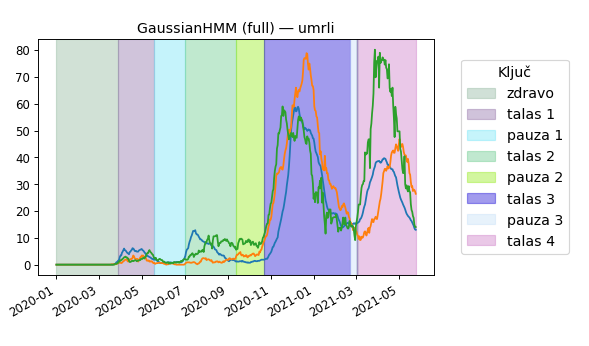
\includegraphics[width=0.8\textwidth]{covid.png}
  \caption{Моделовање тока епидемије \textit{COVID-19} у Републици Србији\cite{vasovic2021}}
  \label{fig:covid}
\end{figure}

Досад је увелико наговештено да су добар избор скривени Марковљеви модели (енгл. \textit{Hidden Markov Model, HMM}), па ће надаље бити речи о њима. Ипак, ваља напоменути се да се наведени проблеми још ефектније решавају својеврсним проширењима \textit{HMM}-а, попут условних случајних поља\cite{ponomareva2007} (енгл. \textit{Conditional Random Field, CRF}), или комбинацијом са другим техникама као што су вештачке неуронске мреже\cite{cohen1999} (енгл. \textit{Artificial Neural Network, ANN}).

% ------------------------------------------------------------------------------
\chapter{Моделовање помоћу \textit{HMM}}
% ------------------------------------------------------------------------------
% Hidden Markov Models
% The Decoding Problem
% Finding the Most Likely Outcome of an HMM
...

% ------------------------------------------------------------------------------
\chapter{Биолошки значај \textit{HMM}}
% ------------------------------------------------------------------------------
% Profile HMMs for Sequence Alignment
% Classifying proteins with profile HMMs
...

% ------------------------------------------------------------------------------
\chapter{Учење \textit{HMM}}
% ------------------------------------------------------------------------------
% Learning the Parameters of an HMM
% Soft Decisions in Parameter Estimation
% Baum-Welch Learning
...

% ------------------------------------------------------------------------------
\chapter{Закључак}
% ------------------------------------------------------------------------------
% The Many Faces of HMMs
% Epilogue: Nature is a Tinkerer and not an Inventor
...

% ------------------------------------------------------------------------------
% Literatura
% ------------------------------------------------------------------------------
\literatura

\end{CJK}
\end{document}